% Main report. Compile on Overleaf with pdfLaTeX (Menu -> Compiler -> pdfLaTeX); BibTeX runs automatically.
\documentclass[11pt,a4paper]{article}

\usepackage[margin=2.5cm]{geometry}
\usepackage[T1]{fontenc}
\usepackage{lmodern}
\usepackage{amsmath,amssymb}
\usepackage{booktabs,tabularx,array}
\usepackage{graphicx}
\usepackage{xcolor}
\usepackage{tikz}
\usetikzlibrary{positioning,arrows.meta}
\usepackage[numbers,sort&compress]{natbib}
\usepackage[colorlinks=true,linkcolor=blue!50!black,citecolor=blue!50!black,urlcolor=blue!50!black]{hyperref}

\graphicspath{{figures/}}

% Marks text that must be filled from experiment results before submission.
\newcommand{\todo}[1]{\textcolor{red}{\textbf{[TODO: #1]}}}
\newcommand{\STOP}{\textsc{stop}}
\newcommand{\CONT}{\textsc{continue}}

\newcommand{\numCqwen}{0.40}
\newcommand{\tDraftQwen}{10.7}
\newcommand{\tTargetQwen}{26.5}
\newcommand{\numCsmol}{0.25}
\newcommand{\tDraftSmol}{6.6}
\newcommand{\tTargetSmol}{26.7}
  % measured constants, written by `uv run python -m specrl.report_tables`
% One-paragraph findings shared by main.tex (report) and slides.tex. Numbers from results/*.csv (10 Nov 2026).

% ---- report ----
\newcommand{\resultsParagraph}{%
All four RL agents beat every baseline on both model pairs, in the simulator and in real wall-clock time.
On the RTX~3050, Value Iteration is fastest: 1.51$\times$ the target alone for Qwen and 1.75$\times$ for
SmolLM2, against 1.42$\times$ and 1.65$\times$ for the best baseline (HuggingFace's 0.4 confidence threshold)
and 1.38$\times$ and 1.57$\times$ for the best fixed draft length. REINFORCE (1.50$\times$ / 1.70$\times$) and DQN
(1.47$\times$ / 1.70$\times$) follow closely; Q-learning is last among the agents (1.47$\times$ / 1.67$\times$) but
still ahead of all baselines. The agents gain \emph{fewer} tokens per target call than the threshold rule yet
are faster: they stop earlier when a rejection is likely and so waste fewer draft steps. Speedups are larger
for SmolLM2, whose draft step is cheaper relative to its target ($c=0.25$ vs $0.40$).}

\newcommand{\heatmapSentence}{%
Value Iteration learned a clean threshold on $q$: it stops whenever the estimated chance that all drafts
survive falls below about 0.7, and continues otherwise. This is the shape SpecDec++~\citep{huang2024specdecpp}
proves optimal, and the agent was not told it: it came out of the Bellman equation. DQN and REINFORCE learned
soft thresholds around $q\approx0.3$--$0.5$; within one cell they sometimes stop and sometimes continue,
because they also read the latest token's confidence $p$ and the entropy $H$, which $q$ does not capture.
Q-learning shows the same idea, but noisily.}

\newcommand{\taskSentence}{%
The agents draft about twice as long on code and maths as on chat (Value Iteration: 2.0 tokens per round on
chat, 4.0--4.2 on code and maths) without being told the task: they read it from the draft's confidence.
Code and maths answers are formulaic (the draft matches the target 92--93\% of the time), chat is open-ended
(78\%). The largest live speedups are on code: 1.61$\times$ for Qwen and 2.03$\times$ for SmolLM2 with Value
Iteration.}

\newcommand{\lambdaSentence}{%
A cheap target call (low $\lambda$) makes the agent draft long rounds and waste rejected drafts; an expensive
one makes it stop early, and at 1.4 times the tuned value it collapses to stopping after a single token, the
failure mode anticipated in our proposal. The best speedup lies exactly at the $\lambda$ chosen by the
Dinkelbach update, which confirms the method.}

\newcommand{\simLiveSentence}{%
The simulator ranks the methods in the same order as the live benchmark (Spearman rank correlation 1.00 for
Qwen, 0.94 for SmolLM2, where DQN and REINFORCE, 0.005$\times$ apart, swap places). Live speedups are 8\%
(Qwen) and 14\% (SmolLM2) lower than simulated, because the simulator does not count the per-step cost of
computing features, querying the policy and Python control flow; that fixed overhead weighs more when the
draft step itself is cheaper (SmolLM2). Training in the simulator is therefore a reliable way to compare and
choose policies, but its absolute speedups are optimistic.}

\newcommand{\hypothesesParagraph}{%
\begin{enumerate}
  \item \emph{All four agents match or beat the best fixed-$k$ baseline}: confirmed, live and simulated, on both pairs.
  \item \emph{Value Iteration is the strongest tabular method and Q-learning approaches it}: confirmed; Value
  Iteration was the strongest method overall.
  \item \emph{DQN and REINFORCE gain from the richer state, with REINFORCE noisier}: partly. Both beat
  Q-learning but not Value Iteration, and with per-round episodes REINFORCE was not noisier.
  \item \emph{The learned policies look like a threshold on $q$}: confirmed (Figure~\ref{fig:heatmap}).
  \item \emph{Speedups are larger on the SmolLM2 pair}: confirmed (1.75$\times$ vs 1.51$\times$ live).
\end{enumerate}}

\newcommand{\seedSentence}{%
Retraining Q-learning, DQN and REINFORCE with three seeds each (Table~\ref{tab:seeds}) confirms the ranking where
the gaps are large: Q-learning is last on both pairs for every seed, and on Qwen the order Value Iteration $>$
REINFORCE $>$ DQN holds for every seed. On SmolLM2, Value Iteration, DQN and REINFORCE lie within each other's
seed ranges (2.01--2.02$\times$), so their differences there are noise.}

\newcommand{\conclusionParagraph}{%
All four algorithms learned useful stopping rules from a simulator built in minutes, and all of them beat
fixed draft lengths and HuggingFace's confidence threshold in real wall-clock time: up to 1.51$\times$
(Qwen) and 1.75$\times$ (SmolLM2) faster than the target model alone, with the same output. Model-based Value
Iteration, the simplest method, was the strongest: with an accurate model of the environment available,
planning beat learning from samples. The agents rediscovered the threshold rule that theory predicts, and
learned on their own to draft longer on predictable code and maths than on open-ended chat.}

% ---- slides ----
\newcommand{\resultsSentence}{All four agents beat every baseline live. Best: Value Iteration, 1.51$\times$
(Qwen) and 1.75$\times$ (SmolLM2) vs 1.42$\times$ / 1.65$\times$ for HuggingFace's threshold rule.}
\newcommand{\heatmapShort}{Value Iteration learned a clean threshold: \STOP{} when $q<0.7$. Nobody told it;
it is the rule SpecDec++ proves optimal. DQN and REINFORCE learned soft versions of it.}
\newcommand{\taskShort}{Agents draft about twice as long on code and maths as on chat, learned from the
draft's confidence alone. Largest live gain: code, 2.03$\times$ (SmolLM2).}
           % one-paragraph findings shared with the slides (written by hand)

\title{Learning When to Stop Drafting:\\Reinforcement Learning for Adaptive Speculative Decoding in LLMs}
\author{
  \textbf{Thapar Institute of Engineering and Technology, Patiala}\\[0.6em]
  \begin{tabular}{ll}
    \toprule
    Name & Roll number \\
    \midrule
    Shikhar Saxena    & 102316078 \\
    Vaibhav Sundriyal & 102316077 \\
    Angad Shukla      & \todo{roll no.} \\
    \bottomrule
  \end{tabular}
}
\date{November 2026}

\begin{document}
\maketitle

\begin{abstract}
We train a reinforcement learning agent that decides, token by token, how long a small draft model should keep drafting before a large target model verifies its guesses. This speeds up LLM text generation while keeping the output identical to the large model's.

Speculative decoding pairs a small, fast draft model with a large target model: the draft proposes several tokens and the target checks them all in one forward pass. The number of tokens drafted per round decides the speedup. Too few and the target is called too often; too many and most drafts are thrown away. Current systems use a fixed draft length or a hand-set confidence threshold.

We model the drafting decision as a Markov Decision Process (MDP) whose state is built from the draft model's confidence signals and whose reward is tokens gained minus the cost of a target call. We solve it with four algorithms that span the course syllabus: Value Iteration (dynamic programming), Q-learning (temporal difference), Deep Q-Network (function approximation and deep RL) and REINFORCE (policy gradient). We train them in a fast simulator built from logged model outputs and evaluate them in a live speculative-decoding loop on two open model pairs (Qwen2.5 0.5B$\to$1.5B and SmolLM2 135M$\to$1.7B) on consumer GPUs, against fixed-length and threshold baselines. All four agents beat every baseline in real wall-clock time. The best, Value Iteration, generates
1.51$\times$ (Qwen) and 1.75$\times$ (SmolLM2) faster than the target model alone, up to 2.03$\times$ on code,
against 1.42$\times$ and 1.65$\times$ for HuggingFace's confidence-threshold rule. The agents rediscover the
threshold-style stopping rule that theory predicts is optimal, and learn on their own to draft longer on code
and maths than on chat.
\end{abstract}

\section{Introduction and motivation}

Large language models generate text one token at a time, and every token needs a full forward pass of the model. On real hardware this step is limited by memory bandwidth, not compute: the GPU spends most of its time loading weights, not doing arithmetic. Checking 5 tokens in one pass therefore costs almost the same as generating 1.

Speculative decoding~\citep{leviathan2023fast,chen2023accelerating} uses this gap. A small model guesses ahead and the large model verifies the guesses in parallel. With greedy decoding the final text is exactly the large model's own output, so speed improves at \textbf{no loss in quality}.

\paragraph{Analogy.} A junior writer (the draft model) quickly drafts a few words, and a senior editor (the target model) checks the whole draft in one read. If the junior writes too little, the editor is interrupted constantly. If the junior writes too much, most of it is crossed out. Our RL agent is the manager who decides, word by word, when the junior should stop and hand the draft over.

The right moment to stop changes all the time. Predictable text such as code boilerplate or a list continuation can be drafted far ahead. A creative sentence or the answer to a maths step should be checked early. A fixed rule cannot adapt to this, but an agent that watches the draft model's confidence can. This makes the problem a natural fit for reinforcement learning: a sequential decision under uncertainty with a clear numeric reward.

\paragraph{Objectives.}
\begin{enumerate}
  \item Formulate draft-length control as an MDP with a reward tied directly to generation throughput.
  \item Solve it with four RL algorithms from the course (Value Iteration, Q-learning, DQN, REINFORCE) and compare them on the same task.
  \item Measure real wall-clock speedups on consumer GPUs against standard baselines.
  \item Inspect what the agents learn, and test whether they discover the threshold-style rule that theory predicts is optimal.
  \item Present the result as a live, visual side-by-side demo.
\end{enumerate}

\section{Background: speculative decoding}

Each round of greedy speculative decoding yields $n+1$ tokens for one target call, where $n$ is the number of drafted tokens the target agrees with.
\begin{enumerate}
  \item The draft model generates tokens $d_1, d_2, \dots, d_k$ one by one (cheap).
  \item The target model runs once on the context plus $d_1 \dots d_k$ and gives its own greedy choice at every position.
  \item Drafts are accepted left to right while they match the target's choice. Call the number accepted $n$.
  \item The target's own token at position $n+1$ is gained for free, either as a correction or as a bonus when all $k$ drafts were accepted.
\end{enumerate}
The result is identical to running the target alone, because every kept token is one the target would have chosen.

\begin{table}[h]
\centering
\caption{Existing rules for choosing the draft length $k$.}
\label{tab:existing-rules}
\begin{tabularx}{\linewidth}{@{}lXX@{}}
\toprule
Rule & How it decides when to stop & Weakness \\
\midrule
Fixed $k$ & Always drafts $k$ tokens (often $k=4$ or $5$) & Ignores how easy the current text is \\
Confidence threshold (HuggingFace)~\citep{hfdynamic} & Stops when the draft's top-token probability falls below 0.4 & One hand-picked number for every model pair and task \\
SpecDec++~\citep{huang2024specdecpp} & Stops when the estimated chance that a draft has already been rejected crosses a threshold & Needs a separately trained acceptance predictor \\
\bottomrule
\end{tabularx}
\end{table}

SpecDec++ shows that the optimal stopping rule is a threshold on the probability that a rejection has already happened. This gives us a theoretical yardstick: a well-trained RL agent should rediscover a threshold-like policy on its own, and we check whether it does.

\section{Problem formulation as an MDP}
\label{sec:mdp}

After every drafted token the agent chooses \CONT{} or \STOP{}. Its reward is the number of tokens gained minus the time cost of the round, measured in tokens.

\begin{table}[h]
\centering
\caption{MDP definition.}
\label{tab:mdp}
\begin{tabularx}{\linewidth}{@{}lX@{}}
\toprule
Part & Definition \\
\midrule
Episode & Generating the full answer (e.g.\ 128 tokens) for one prompt, made of many draft$\to$verify rounds \\
State & $s$ = tokens drafted so far this round (1--8); $p$ = top probability of the latest draft token; $H$ = entropy of the draft distribution; $q$ = product of $p$ over this round (estimated chance that all drafts survive); $a$ = moving average of the recent acceptance rate \\
Actions & \CONT{} (draft one more token) or \STOP{} (send to the target). \STOP{} is forced at $s = K = 8$ \\
Reward & 0 on \CONT{}. On \STOP{}: $r = (\min(s,n)+1) - \lambda(1 + s\,c)$ \\
Discount & $\gamma = 1$ (episodic and bounded), or $0.99$ for stability with DQN and REINFORCE \\
\bottomrule
\end{tabularx}
\end{table}

Here $c = t_\text{draft} / t_\text{target}$ is the measured cost of one draft step relative to one target call, and $\lambda$ is the price of one target call in tokens. \todo{measured values of $c$ for each model pair.}

\paragraph{Choosing $\lambda$.} Maximising throughput (tokens per unit time) is a ratio objective. By Dinkelbach's method~\citep{dinkelbach1967} it equals maximising $\text{tokens} - \lambda\cdot\text{time}$, where $\lambda$ is the best achievable throughput. In practice we set $\lambda$ to the throughput of the best fixed-$k$ baseline, train, measure the new throughput, update $\lambda$ and retrain once. We also report a small sweep over $\lambda$.

\paragraph{Bellman optimality equations.}
\begin{align}
Q^*(s,\STOP) &= \mathbb{E}\left[\min(s,n)+1\right] - \lambda(1+s\,c) + \gamma\,\mathbb{E}\left[V^*(s_{\text{next round}})\right] \\
Q^*(s,\CONT) &= \gamma\,\mathbb{E}\left[\max_{a'} Q^*(s',a')\right] \\
V^*(s) &= \max\left(Q^*(s,\STOP),\; Q^*(s,\CONT)\right)
\end{align}
For the tabular methods the next-round term is the same under both actions, so each round can be treated as a short episode of at most 8 steps.

\section{Methods: four RL algorithms}

We solve the same MDP with four algorithms, chosen so that each pair of them contrasts one idea from the course~\citep{sutton2018}.

\begin{table}[h]
\centering
\caption{The four algorithms and their final settings.}
\label{tab:algos}
\small
\begin{tabularx}{\linewidth}{@{}l>{\raggedright}p{2.4cm}>{\raggedright}p{2.8cm}X@{}}
\toprule
Algorithm & Course topic & State & Key details \\
\midrule
Value Iteration & Dynamic programming, Bellman equations & Tabular: $s$ (1--8) $\times$ 10 bins of $q$ = 80 states & Transition probabilities and expected rewards counted from the logs (every logged position as a round start), then Bellman optimality updates until the residual is below $10^{-9}$ (about 8 sweeps) \\
Q-learning & Temporal-difference learning & Same 80 tabular states & $Q(s,a) \leftarrow Q(s,a) + \alpha[r + \max_{a'} Q(s',a') - Q(s,a)]$, $\alpha=0.05$, $\varepsilon$-greedy ($1\to0.05$ over 80\% of training), 10\,000 episodes \\
DQN~\citep{mnih2015} & Function approximation, deep RL & Continuous features $[s/8, p, H/5, q, a]$ & MLP 5$\to$64$\to$64$\to$2, replay buffer of 50k steps, batch 128, update every 4 steps, target network synced every 500 steps, Huber loss, Adam ($10^{-3}$), 3000 episodes \\
REINFORCE~\citep{williams1992} & Policy gradient & Same continuous features & Softmax policy MLP 5$\to$64$\to$2, Monte Carlo returns, mean-return baseline, advantages divided by their standard deviation, Adam ($10^{-3}$), 3000 episodes \\
\bottomrule
\end{tabularx}
\end{table}

\paragraph{Episodes.} All four algorithms treat each draft$\to$verify round as one short episode of at most
8 decisions with $\gamma=1$: \CONT{} bootstraps from the next state of the same round, and \STOP{} ends it.
An answer has a fixed number of tokens whatever the policy, so a whole-answer return would only measure
time and $\lambda$ would have no effect. Per round, maximising
$\mathbb{E}[\text{gained}-\lambda\,\text{cost}]$ is exactly Dinkelbach's form of maximising throughput.
Steps where \STOP{} is forced ($s=8$, end of the answer) are stored as \STOP{} and get no policy gradient,
and \CONT{} at $s=8$ is excluded from bootstrap targets.

\paragraph{Choosing $\lambda$.} Each algorithm is trained twice: first with $\lambda$ equal to the best
fixed-$k$ throughput on the training prompts, then with $\lambda$ equal to the throughput its own first policy
reached (one Dinkelbach update).

\paragraph{Comparison axes.}
\begin{itemize}
  \item Model-based (Value Iteration) vs model-free (Q-learning).
  \item Tabular (Q-learning) vs function approximation (DQN).
  \item Value-based (DQN) vs policy-based (REINFORCE).
\end{itemize}

\paragraph{Baselines (not RL).}
\begin{itemize}
  \item Target model alone, with no speculation (speedup $= 1.0\times$ by definition).
  \item Fixed draft length $k = 1$ to $8$.
  \item Confidence threshold: stop when $p < 0.4$, as in HuggingFace's dynamic speculation~\citep{hfdynamic}.
\end{itemize}

\section{System design}

The GPU is used only twice: once to log model outputs and once for the final live benchmark. All RL training runs on the CPU in a simulator built from those logs (Figure~\ref{fig:pipeline}).

\begin{figure}[h]
\centering
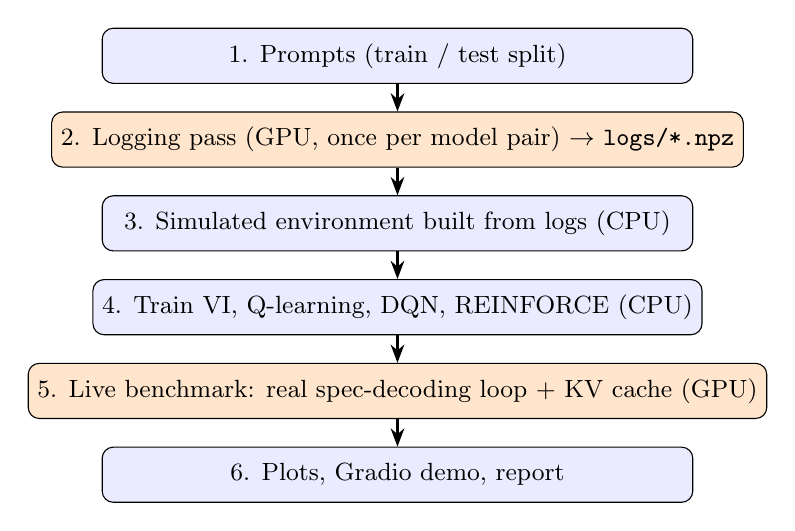
\begin{tikzpicture}[
  node distance=0.35cm,
  box/.style={draw, rounded corners, minimum width=7.5cm, minimum height=0.7cm, align=center, font=\small},
  gpu/.style={box, fill=orange!20},
  cpu/.style={box, fill=blue!8},
  arr/.style={-{Stealth}, thick}]
\node[cpu] (a) {1. Prompts (train / test split)};
\node[gpu, below=of a] (b) {2. Logging pass (GPU, once per model pair) $\to$ \texttt{logs/*.npz}};
\node[cpu, below=of b] (c) {3. Simulated environment built from logs (CPU)};
\node[cpu, below=of c] (d) {4. Train VI, Q-learning, DQN, REINFORCE (CPU)};
\node[gpu, below=of d] (e) {5. Live benchmark: real spec-decoding loop + KV cache (GPU)};
\node[cpu, below=of e] (f) {6. Plots, Gradio demo, report};
\foreach \x/\y in {a/b,b/c,c/d,d/e,e/f} \draw[arr] (\x) -- (\y);
\end{tikzpicture}
\caption{System pipeline. Only the orange steps need the GPU.}
\label{fig:pipeline}
\end{figure}

\paragraph{Smart logging.} With greedy decoding the final text is the same for every policy, since it is always the target's greedy output. So for each prompt we:
\begin{enumerate}
  \item Generate the target's greedy answer once (8 prompts per batch; repetition penalty off, so the text is pure greedy).
  \item Run one forward pass of the draft model over the full text.
  \item Store, at every position $t$, the draft's top probability $p_t$, its entropy $H_t$, and $\text{match}_t$ = whether the draft's top token equals the true next token.
\end{enumerate}
In the simulator, a round that starts at position $t$ with $s$ drafts accepts $n$ = the number of consecutive matches from $t$, capped at $s$. Any policy can therefore be replayed at any round start without re-running the language models. Logging costs two forward passes per prompt and takes minutes.

One approximation remains: after the first wrong draft token, a real draft model would continue from its own mistake, while the log continues from the true text. Those tokens are rejected anyway, and the live benchmark checks that the gap is small.

\paragraph{Live benchmark.} A real draft$\to$verify loop with a key-value cache. Each model keeps a fixed-size cache and one recorded CUDA graph per input length (1--10 tokens), which removes the per-step kernel-launch overhead; after each verify the cache position is moved back to the accepted length, so rejected drafts are forgotten. The target-alone baseline uses the same machinery. Correctness test: the output must equal the target's own greedy output on 20 test prompts. Timing uses 3 warm-up runs, CUDA synchronisation, and 3 timed runs.

\begin{table}[h]
\centering
\caption{Models and hardware.}
\label{tab:models}
\small
\begin{tabularx}{\linewidth}{@{}lXll@{}}
\toprule
Where & Draft $\to$ Target & VRAM (fp16, est.) & Role \\
\midrule
Laptop (RTX 3050, 6\,GB) & Qwen2.5-0.5B-Instruct $\to$ Qwen2.5-1.5B-Instruct & $\sim$4.5\,GB & Main pair \\
Laptop (RTX 3050, 6\,GB) & SmolLM2-135M-Instruct $\to$ SmolLM2-1.7B-Instruct & $\sim$4\,GB & 12$\times$ size gap, demo \\
\bottomrule
\end{tabularx}
\end{table}

Draft and target in each pair share a tokenizer, which speculative decoding requires.

\paragraph{Data.} 498 prompts mixed from Alpaca (167 chat instructions), HumanEval (all 164 code problems) and GSM8K (167 maths questions), so results can be compared per task type. 20\% of each task (99 prompts) is held out as the test set; agents train on the other 399.

\section{Experimental setup}

The main measure is real wall-clock speedup over the target model alone, measured on the same machine. The other metrics explain where that speedup comes from.

\begin{table}[h]
\centering
\caption{Metrics.}
\label{tab:metrics}
\begin{tabularx}{\linewidth}{@{}lX@{}}
\toprule
Metric & Meaning \\
\midrule
Speedup & Tokens/sec of a method $\div$ tokens/sec of the target alone (live, same PC) \\
Mean accepted length & Average tokens gained per target call ($n+1$) \\
Simulated reward & Average episode reward in the simulator, on train and test prompts \\
Training cost & Episodes and wall time each algorithm needs to converge \\
Simulation-vs-live gap & Whether the simulator ranks methods in the same order as the live benchmark \\
\bottomrule
\end{tabularx}
\end{table}

\paragraph{Hypotheses.}
\begin{enumerate}
  \item All four RL agents will match or beat the best fixed-$k$ baseline, because they can adapt draft length to the text.
  \item Value Iteration will be the strongest tabular method, since it plans with an estimated model, and Q-learning will approach it with enough samples.
  \item DQN and REINFORCE will gain from the richer continuous state (entropy, acceptance rate), with REINFORCE showing noisier training.
  \item The learned policies will look like a threshold on $q$, matching the theory.
  \item Speedups will be larger on the SmolLM2 pair (12$\times$ size gap) than on the Qwen pair (3$\times$ gap).
\end{enumerate}

\todo{hardware details of the benchmark PC, software versions (PyTorch, transformers, CUDA), training hyperparameters.}

\section{Results}
% Filled after phases P6-P7. Numbers come from results/*.csv; figures from figures/.

\begin{table}[h]
\centering
\caption{Main results. \todo{fill from \texttt{results/*.csv}.}}
\label{tab:main-results}
\small
\begin{tabular}{@{}lcccc@{}}
\toprule
Method & Speedup (Qwen) & Speedup (SmolLM2) & Mean accepted length & Sim reward \\
\midrule
Target alone        & 1.00$\times$ & 1.00$\times$ & 1.00 & -- \\
Fixed $k=4$         & & & & \\
Best fixed $k$      & & & & \\
Threshold 0.4       & & & & \\
Value Iteration     & & & & \\
Q-learning          & & & & \\
DQN                 & & & & \\
REINFORCE           & & & & \\
\bottomrule
\end{tabular}
\end{table}

\paragraph{Training curves.} \todo{Figure: reward vs episodes, all four algorithms.}

\paragraph{What the agent learned.} \todo{Figure: policy heatmap over $(s, q)$. Does it form a threshold, as SpecDec++ predicts?}

\paragraph{Per-task behaviour.} \todo{Does the agent draft longer on code than on chat? Per-task table.}

\paragraph{Effect of $\lambda$.} \todo{$\lambda$ sweep figure.}

\paragraph{Transfer.} \todo{Does a policy trained on the Qwen pair work on the SmolLM2 pair?}

\paragraph{Simulator vs live.} \todo{Do both rank the methods the same way?}

\paragraph{Hypotheses revisited.} \todo{Which of the five hypotheses held.}

\section{Live demo}

The centrepiece is a live race: the same prompt typed once, two panes generating side by side, one with the target alone and one with the RL agent, each with a live tokens-per-second counter. It uses the SmolLM2 pair.

\begin{itemize}
  \item \textbf{Coloured tokens:} green = accepted draft, red = rejected draft, a marker wherever the agent pressed \STOP{}.
  \item \textbf{Confidence meter:} a live bar of the draft model's confidence next to the agent's decision.
\end{itemize}

\todo{screenshot of the demo.}

\section{Related work and our contribution}

Learning the draft length is an active research topic. Our contribution is a controlled, side-by-side comparison of four classic RL families on the same task, run on consumer hardware, with a simulator and a live demo.

\begin{table}[h]
\centering
\caption{Related work.}
\label{tab:related}
\small
\begin{tabularx}{\linewidth}{@{}>{\raggedright}p{3.6cm}XX@{}}
\toprule
Work & Approach & Relation to this project \\
\midrule
Leviathan et al.~\citep{leviathan2023fast}; Chen et al.~\citep{chen2023accelerating} & Original speculative decoding and speculative sampling & The decoding scheme we control \\
SpecDec++~\citep{huang2024specdecpp} & Draft length as an MDP; proves a threshold stopping rule is optimal & Theory our learned policies are checked against \\
Learning to Draft~\citep{ltd2026} & RL that learns draft depth with a throughput reward & Closest prior work. We compare DP, TD, DQN and policy gradient side by side on small models \\
DISCO~\citep{mamou2024disco} & A classifier that picks the draft length each round & Supervised alternative to RL \\
BanditSpec~\citep{banditspec2025} & Bandit algorithms (UCB, EXP3) choose the speculation length & Simpler, state-free alternative \\
HuggingFace dynamic speculation~\citep{hfdynamic} & Stops drafting when confidence $< 0.4$ & Our threshold baseline \\
\bottomrule
\end{tabularx}
\end{table}

\section{Conclusion}

This project applies the full course syllabus (MDPs, Bellman equations, dynamic programming, temporal-difference learning, function approximation, deep Q-learning and policy gradients) to a live problem in LLM inference. The task has a measurable payoff: faster text generation with identical output.

The smart-logging simulator keeps the GPU cost low and lets all four algorithms train in minutes on a laptop CPU. The live benchmark and race demo then show the result on real hardware. \todo{rewrite with the actual findings: which algorithm won, by how much, and whether the threshold policy emerged.}

\paragraph{Limitations.} \todo{e.g.\ greedy decoding only, small models, simulator approximation after the first rejected draft.}


\bibliographystyle{plainnat}
\bibliography{references}

\end{document}
